\documentclass{report}
\usepackage[T1]{fontenc}
\usepackage[utf8]{inputenc}
\usepackage[french]{babel}
\usepackage{color}
\usepackage{amsmath}
\usepackage{amssymb}
% Pour utiliser le signe €
\usepackage{eurosym}
% Pour pouvoir insérer des images
\usepackage{graphicx}
\graphicspath{images/}
% Pour pouvoir insérer des hyperliens
\usepackage[hyphens]{url}
\usepackage{hyperref}
% Suppression des marges supplémentaires sur les bords
\usepackage{fullpage}
% Forcer l'affichage des figures à un endroit précis
\usepackage{here}
% On ne veut pas afficher le mot 'Chapitre' avant chaque chapitre
\usepackage{titlesec}
\titleformat{\chapter}[hang]{\bf\huge}{\thechapter}{2pc}{}

% Pour les en-têtes et pieds de page
\usepackage{fancyhdr}
\renewcommand{\headrulewidth}{0pt}
\lhead{} 
\chead{} 
\rhead{} 
\renewcommand{\footrulewidth}{0.1pt}
\lfoot{Antoine Augusti} 
\cfoot{\thepage} 
\rfoot{\href{http://statistics.teen-quotes.com}{statistics.teen-quotes.com}} 
\pagestyle{fancy}

% Pour forcer l'affichage des en-têtes et pieds de page sur les premières pages des chapitres
\makeatletter
\let\ps@plain\ps@fancy
\makeatother

% Pour barrer du texte
\newlength{\textlarg}
\newcommand{\barre}[1]{%
   \settowidth{\textlarg}{#1}
   #1\hspace{-\textlarg}\rule[0.5ex]{\textlarg}{0.5pt}}

% Coloration syntaxique
\usepackage{listings}
\lstset{ 
	language=SQL,
	numbers=none,
	showstringspaces=false,
	keywordstyle=\color{blue},
	tabsize=4,
	breaklines=true,
	extendedchars=true,
	literate={é}{{\'e}}1 {à}{{\'a}}1 {è}{{\`e}}1 {ç}{{\c c}}1
}
%----------------------- %
% -- Cheat sheet -------- %

% Alignement
%\begin {flushleft}
%\begin {center}
%\begin {flushright}

% Listes
% \begin{itemize}
% \begin{description}
% \begin{enumerate}
% 	\item Numéro 1
% 	\item Numéro 2
% \end{enumerate}
% \\
% \newpage

% Mise en forme des caractères
% \normalfont{} ou \begin{rm}
% \textbf{} ou \begin{bf}
% \textit{} ou \begin{it}
% \textsc{} ou \begin{sc}
% Emphase (sémantique)
% \emph{}

% Citations et code brut
% \quote Pour une ligne isolée
% \quotation Pour un bloc
% \verb Pour du code
% \lstlisting Pour du code coloré

% URL
% \url{http://www.site.org/}
% ------------------------------------ %


% ------------------------------------ %
% -- METADONNÉES DU DOCUMENT --------- %
% Utilisées pour générer la page de garde
\title{
		Projet Final de M8\\
		Étude de Teen Quotes
}
\author{
	Antoine \textsc{Augusti}, 
}
\date{Juin 2013}
\begin{document}

	% Génération de la page de garde
	\maketitle

	% Génération de la table des matières
	\tableofcontents

	% ///////////////////////////////////////////////////////// %
	% /// Introduction //////////////////////////////////////// %
	\chapter{Introduction}
	% ------------------------------------------- %
	% -- Teen Quotes, qu'est-ce que c'est ? ----- %
	\section{Teen Quotes, qu'est-ce que c'est ?}
	Teen Quotes est une plateforme regroupant des citations décrivant le quotidien des adolescents. L'adolescence est une période difficile à gérer dans la vie et les adolescents ont souvent besoin d'échanger autour de sujets qui les préoccupent : leurs amis, l'amour, les études, leurs déceptions, leurs expériences. Teen Quotes répond à ce besoin en proposant à toute personne possédant un compte de pouvoir partager son impression en écrivant une courte citation. Cette citation sera ensuite acceptée (modifiée légèrement ou non) pour publication ou rejetée. Actuellement, cinq nouvelles citations sont publiées tous les jours à 0h (heure française) sur Teen Quotes.\\

	L'interface de Teen Quotes est proposée par défaut en anglais. L'interface est également disponible en français pour ceux qui le désirent et une version en français par défaut existe (elle se nomme Kotado). Toutefois, la version française de Teen Quotes ayant moins de succès que la version originale, j'ai choisi d'orienter mon projet de M8 vers cette version anglaise.\\

	Teen Quotes a été lancé en mai 2011, après quelques mois de développement que j'ai mené seul. Aujourd'hui Teen Quotes possède une version web pour les ordinateurs, une version optimisée pour les smartphones (depuis navigateur) ainsi qu'une application iPhone / iTouch que l'on peut télécharger depuis l'App Store d'Apple. \textbf{Plus de 1,5 million de personnes ont visité Teen Quotes}, depuis l'une des versions que nous proposons.\\

	Je me suis également associé depuis deux ans à une jeune femme philippine (parlant anglais) qui tient le compte Twitter de Teen Quotes (\href{http://twitter.com/ohteenquotes}{\textit{@ohteenquotes}}) comptant actuellement \textbf{plus de 2 millions de followers}. Nous essayons ensemble d'avoir une convergence vers tous les supports où Teen Quotes est présent (Twitter, Facebook, site web, site mobile, application iPhone / iTouch) pour agrandir notre masse d'utilisateurs.

	% ---------------------------------------------------- %
	% -- Et moi, je peux avoir accès à Teen Quotes ? ----- %
	\section{Et moi, je peux avoir accès à Teen Quotes ?}
	Bien évidemment ! Teen Quotes est ouvert à tout le monde et mon but est que le plus de monde possible rejoigne l'aventure. Teen Quotes peut être consulté grâce aux moyens suivants :
	\vspace{10px}
	\begin{itemize}
		\item Site web : \url{http://teen-quotes.com}
		\item Site mobile \footnote{Lien à visiter depuis un smartphone ou une tablette. La redirection vers la version mobile est automatique quand on tente de visiter le site classique depuis un smartphone ou une tablette.} : \url{http://m.teen-quotes.com}
		\item Application iPhone / iTouch \footnote{Lien à visiter depuis un iPhone ou un iTouch pour lancer le téléchargement de l'application !} : \url{http://teen-quotes.com/apps}
	\end{itemize}

	% ---------------------------------------------------- %
	% -- Des données oui, mais des données à jour -------- %
	\section{Des données oui, mais des données à jour}
	Teen Quotes enregistre plus de \textbf{4 000 visites par jour}. Les bases de données de Teen Quotes enregistrent environ \textbf{30 000 requêtes par heure}. Avec un tel volume de données, difficile de se contenter d'une étude statistique figée, obsolète une semaine plus tard car les données ne sont plus du tout les mêmes. Teen Quotes est vivant, évolue en permanence : l'étude statistique de Teen Quotes doit s'adapter en conséquence.\\

	En réponse à ce défi, j'ai décidé d'orienter mon projet de M8 vers une étude statistique évolutive, qui se renouvelle en permanence et qui a pour ambition de donner des informations correctes et précises en quasi temps réel. Pour répondre à ce besoin, quoi de mieux que de proposer une étude en ligne ? Facile à consulter : il suffit d'un navigateur web.

	% Comment ça fonctionne ?
	\subsection{Comment ça fonctionne ?}
	L'idée était donc de créer une partie du site de Teen Quotes dédiée aux statistiques : affichage de graphiques et informations sur les données. Les données sont recalculées 3 fois par heure (soit \textbf{toutes les 20 minutes} si vous suivez !). La réflexion suivie pour arriver à ceci a donc été la suivante :
	\vspace{10px}
	\begin{enumerate}
		\item Quelles sont les données que je veux afficher ?
		\item Comment est-ce que je peux récupérer ces données ? Sont-elles enregistrées dans mes bases de données ou sur un service externe (Google Analytics \footnote{Google Analytics fournit une analyse d'audience pour le site web classique et le site web mobile.}, Flurry \footnote{Flurry fournit des données sur les utilisateurs de l'application iPhone / iTouch.}) ?
		\item Comment faut-il rassembler les données ? Comment donner du sens aux données brutes ? Comment les formater ?
		\item Comment proposer un affichage agréable et lisible pour donner sens aux données récupérées ?
		\item Comment automatiser tout ce processus pour pouvoir effectuer une mise à jour des informations toutes les 20 minutes ?
	\end{enumerate}
	\vspace{10px}
	Le résultat final est visible à l'adresse \url{http://statistics.teen-quotes.com} et est disponible en anglais (dans un souci d'intérêt pour le public visé par Teen Quotes !) et en français. Je vous invite fortement à vous rendre à cette adresse, la suite du rapport expliquant en détail chaque graphique affiché sur cette page.\\

	Des précisions techniques seront apportées au fur et à mesure du rapport pour vous faire une idée de comment est réalisée cette page. Programme alléchant, non ? Allez hop, en voiture, plongeons-nous dans les données !

	% ///////////////////////////// %
	% /// Halte ! Qui va là ? ///// %
	\chapter{Halte ! Qui va là ?}
	Quand nous avons décidé de lancer Teen Quotes, nous ne savions qu'une chose : il fallait que le site soit en anglais pour toucher le plus de monde possible à travers le globe. Partout dans le monde où il y avait un accès à Internet et où les gens parlaient anglais, nous devions pouvoir être accessibles.\\

	Nous n'avions pas une population cible précise et pas de préférence particulière pour un ou des pays. La communication n'a jamais été orientée vers une quelconque culture ou un quelconque continent. Les statistiques obtenues sont donc une régulation naturelle des flux vers Teen Quotes.

	% ------------------------------------------ %
	% -- Où habites-tu petit visiteur ? -------- %
	\section{Où habites-tu petit visiteur ?}
	La première chose à déterminer est la localisation géographique de connexion des visiteurs pour accéder à Teen Quotes. Ceci nous permet d'avoir en notre possession plusieurs informations importantes :
	\vspace{10px}
	\begin{itemize}
		\item Une connaissance de notre audience dans l'éventualité de s'orienter plus vers un pays ou un continent pour des opérations futures.
		\item Un besoin d'optimisation technique vers les pays de grande audience : nos serveurs sont en France mais très peu de visiteurs visitent Teen Quotes depuis la France.
	\end{itemize}
	\vspace{10px}
	Les données de localisation des visites sont données par Google Analytics pour le site web et le site pour mobiles. Les données de localisation pour l'application iPhone / iTouch sont fournies par Flurry. Flurry se contente de donner des informations au niveau des continents alors que Google Analytics est capable de déterminer la localisation au niveau des villes de taille moyenne (Rouen par exemple). Dans un souci de respect de la vie privée des utilisateurs, on se limite à une localisation au niveau de la ville moyenne la plus proche de son lieu de connexion.\\

	On s'intéresse à la totalité des visites de Teen Quotes depuis la création en mai 2011 jusqu'en juin 2013 : on compte donc des personnes en double, forcément. Toutefois il est impossible de faire autrement : les visiteurs peuvent se déplacer géographiquement, changer d'adresse IP... La seule solution pour éviter les doublons serait de ne s'intéresser qu'aux visites de personnes authentifiées sur Teen Quotes, ce qui nous priverait d'une bonne partie des données.\\

	Comme on souhaite s'intéresser aux visites par pays, on ne retient que les données de localisation du site web et du site optimisé pour mobiles en laissant de côté les données de localisation de l'application iPhone / iTouch qui a été lancée en novembre 2012.
	\begin{figure}[H]
		\center
		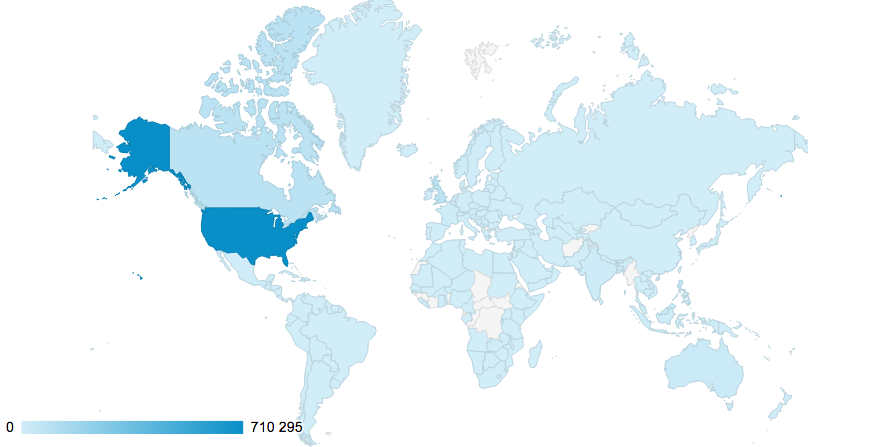
\includegraphics[width=400px]{images/visitesMondialesCarte.png}
		\caption{Visites depuis la création de Teen Quotes représentées sur une carte mondiale.}
	\end{figure}
	On a appliqué un dégradé de bleu pour symboliser le nombre de visites : le bleu foncé représentant le pays avec le plus de visiteurs.\\
	De cette carte on peut tirer l'analyse suivante :
	\vspace{10px}
	\begin{itemize}
		\item Quasiment tous les pays du monde sont coloriés en bleu : c'est-à-dire qu'il y a eu au moins une visite depuis 211 pays ou États\footnote{On obtient ce chiffre en regardant la liste des pays qui ont enregistré au moins une visite, et non en les comptant sur la carte !} dans le monde. Les pays grisés sont majoritairement situés en Afrique : l'absence de visites depuis ces pays peut s'expliquer par le faible taux d'accès à Internet pour les particuliers.
		\item Les visites depuis les États-Unis ont l'air très majoritaires, à tel point qu'il est difficile de voir une différence pour les autres visites tant les écarts sont grands entre le pays le plus visité et les autres.
	\end{itemize}
	\vspace{10px}
	Pour mieux visualiser le poids de chaque pays, représentons les visites sur un diagramme circulaire.
	\begin{figure}[H]
		\center
		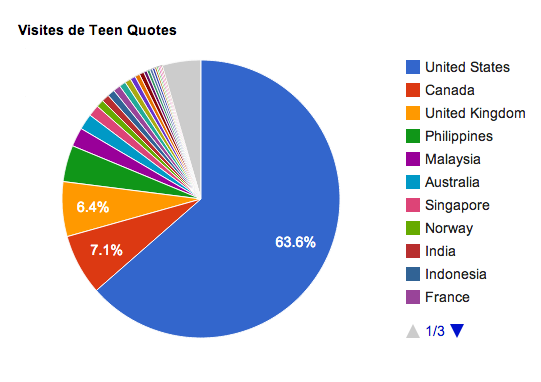
\includegraphics[width=250px]{images/visitesMondialesCamembert.png}
		\caption{Visites depuis la création de Teen Quotes représentées sur un diagramme circulaire.}
	\end{figure}
	La tendance observée précédemment est confirmée : les États-Unis sont de loin le pays qui génère le plus de visites. Plus impressionnant encore \textbf{le top 5 des pays (États-Unis, Canada, Royaume-Uni, Philippines et Malaisie) totalise 83,5 \% du total des visites}. Le reste des pays est très dispersé, contribuant chacun à environ 1 \% des visites.

	% ------------------------------------------ %
	% -- Plutôt smartphones ou ordinateurs ? --- %
	\section{Plutôt smartphones ou ordinateurs ?}
	On a vu précédemment que l'application pour iPhone / iTouch a été lancée en novembre 2012 alors que le site web et la version mobile ont été lancés en mai 2011. Pourquoi avoir attendu autant ? Tout simplement parce qu'il s'est avéré nécessaire en observant les données au fil du temps de posséder une telle application. Retour sur cette décision !\\

	Ici nous allons nous intéresser à l'évolution du nombre de visites par mois depuis un ordinateur, un mobile (smartphone ou tablette) et depuis l'application iPhone / iTouch quand celle-ci a été lancée.
	\begin{figure}[H]
		\center
		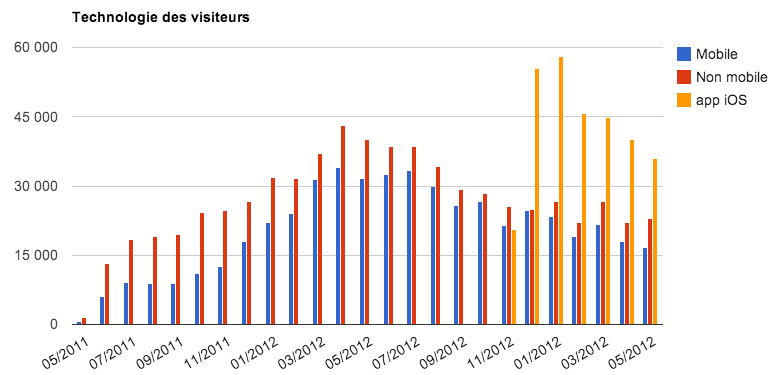
\includegraphics[width=500px]{images/visitesParAppareil.png}
		\caption{Visites mensuelles par type d'appareil.}
	\end{figure}
	Interprétons maintenant les résultats obtenus :
	\vspace{10px}
	\begin{itemize}
		\item Avant le lancement de l'application iOS on remarque qu'il y a quasiment autant de visiteurs depuis un appareil mobile que depuis un ordinateur. Cette statistique suit la montée du mobile dans les usages du web mais dans des proportions importantes : plus de 40 \% des visites se font depuis un smartphone ou une tablette. C'est cette statistique qui nous a poussé à réaliser une application iPhone / iTouch.
		\item Après le lancement de l'application iPhone / iTouch, pratiquement 50 \% des visites se font depuis l'application ! Le succès est grand. Le faible succès au mois de novembre 2012 s'explique par le lancement en fin de mois de l'application.
	\end{itemize}
	\vspace{10px}
	Maintenant, posons-nous la question : \textbf{pourquoi une application pour iOS et pas pour Android ou Windows Phone ?} Intéressons-nous aux systèmes d'exploitation mobiles qui ont navigué sur Teen Quotes.
	\begin{figure}[H]
		\center
		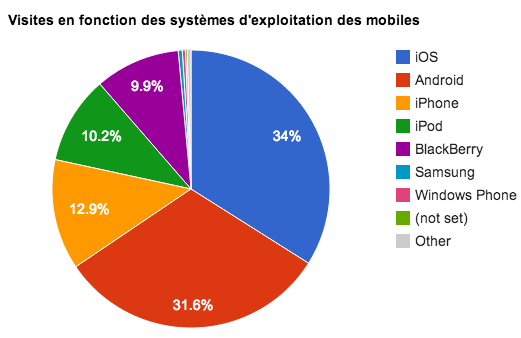
\includegraphics[width=300px]{images/OSMobiles.png}
		\caption{Visites en fonction des systèmes d'exploitation des mobiles.}
	\end{figure}
	En regardant ce diagramme, on pourrait penser que iOS est juste devant Android, sans une grande longueur d'avance. La subtilité réside dans le fait que le système d'exploitation des iPhone et iTouch est en réalité iOS : ces appareils annonçaient un nom différent il n'y a pas encore si longtemps. Il faut donc ajouter les pourcentages attribués aux systèmes d'exploitation iPhone et iTouch à iOS.\\

	Au final, on arrive à 57,1 \% des appareils mobiles sous iOS contre 31,6 \% des appareils mobiles sous Android. L'explication est donc là : \textbf{pour proposer une application qui répondait le plus aux attentes de nos visiteurs il fallait créer une application pour iOS}.
	\newpage
	% ---------------------------------------------- %
	% -- On ne passe pas assez de temps ensemble --- %
	\section{On ne passe pas assez de temps ensemble}
	Plus un visiteur reste longtemps, plus je suis content. J'aime bien quand les visiteurs prennent le temps de lire plusieurs citations voire plusieurs pages de citations ! Le top de mon bonheur étant bien sûr la création d'un compte voire même le remplissage d'un profil. Le comble du bonheur... Mais je m'éloigne du sujet il me semble : la durée moyenne de visite d'un visiteur de Teen Quotes.\\

	Observons donc l'évolution de la durée de visite moyenne d'un visiteur par mois depuis la création de Teen Quotes.
	\begin{figure}[H]
		\center
		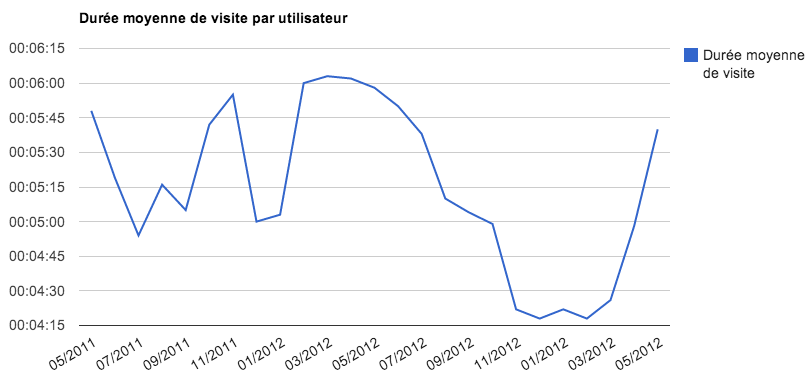
\includegraphics[width=500px]{images/dureeVisite.png}
		\caption{Durée de visite moyenne d'un visiteur.}
	\end{figure}
	On remarque immédiatement que la durée moyenne de visite la plus basse est de plus de 4 minutes et 15 secondes. C'est une excellente moyenne pour un site web ! Bonne nouvelle : Teen Quotes arrive à retenir les visiteurs pendant plusieurs minutes. N'oublions pas que plus de 40 \% des visites sont réalisées depuis un appareil mobile où la durée d'attention est généralement réduite.\\

	On remarque que les données sont assez éparpillées : il y a un écart de quasiment 2 minutes entre la valeur minimale et la valeur maximale ! Et 2 minutes de durée de visite en moyenne de différence sur une période d'un mois, c'est beaucoup. Je n'ai pas encore trouvé d'explication à ces écarts, je tâcherai de surveiller particulièrement ceci à l'avenir.

	% ------------------------------------- %
	% -- C'est un garçon ou une fille ? --- %
	\section{C'est un garçon ou une fille ?}
	J'ai bien peur d'avoir accouché de plusieurs millions de filles. Enfin pas vraiment moi, mais plutôt Teen Quotes ! La connaissance de l'audience passe aussi par le genre des visiteurs : on ne proposera pas les mêmes citations à un public majoritairement féminin que masculin. Il est donc primordial de savoir quelle est la proportition de femmes et d'hommes dans notre audience.\\

	Les données proviennent des informations recueillies sur tous les utilisateurs de l'application iPhone / iTouch et des utilisateurs ne s'étant pas inscrits depuis l'application ayant renseigné leur sexe dans le profil de leur compte Teen Quotes. En effet, Flurry permet de connaître le sexe de l'utilisateur grâce aux informations de son compte Apple alors qu'il n'y a pas de moyen technique permettant d'identifier le sexe d'un visiteur naviguant sur le web !
	\begin{figure}[H]
		\center
		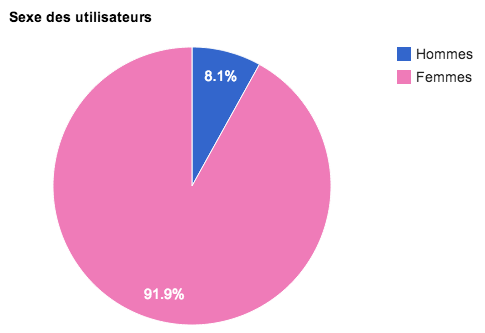
\includegraphics[width=300px]{images/sexeUtilisateurs.png}
		\caption{Proportion d'hommes et de femmes visitant Teen Quotes.}
	\end{figure}
	Wahou, c'est un non-match : il y a un paquet de filles. En y réfléchissant ceci peut se comprendre : les filles ont général plus besoin de se confier et de s'identifier que les garçons lors de la période de l'adolescence. Ça tombe bien, c'est exactement ce pourquoi a été créé Teen Quotes ! En plein dans le mille.

	% ///////////////////////////////////// %
	% /// Des citations, par milliers ///// %
	\chapter{Des citations, par milliers}
	Avant de s'attarder sur le coeur de Teen Quotes (les citations), il convient de rappeller les quelques subtilités associées à celles-ci. Par commodité, on appelle les citations de Teen Quotes les \textbf{« quotes »}.
	\vspace{10px}
	\begin{itemize}
		\item Chaque utilisateur possédant un compte sur Teen Quotes peut soumettre 5 quotes par jour.
		\item Une fois une citation soumise, elle doit être acceptée avant d'être publiée. Une citation peut être acceptée telle qu'elle a été soumise ou légèrement modifiée.
		\item Tous les soirs à 0h (heure française), 5 nouvelles citations sont publiées.
		\item Il existe un système de « file d'attente » qui regroupe les citations en attente de publication : les citations ayant été approuvées les premières étant publiées en priorité.
	\end{itemize}

	% ----------------------------------------- %
	% -- Les statuts des quotes (Statu quo) --- %
	\section{Les statuts des quotes (\textit{Statu quo})}
	Intéressons-nous d'abord aux proportions des différents statuts de quotes.
	\begin{figure}[H]
		\center
		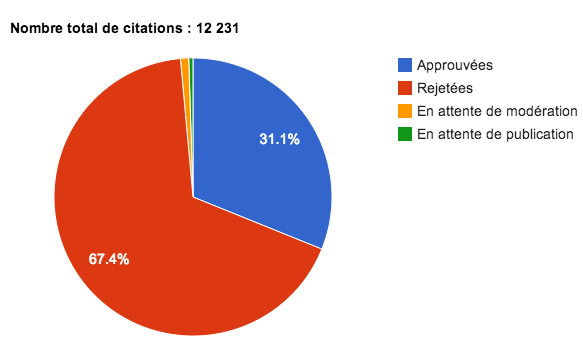
\includegraphics[width=330px]{images/statutsQuotes.png}
		\caption{Parts des différents statuts des quotes sur Teen Quotes.}
	\end{figure}
	On remarque qu'une majeure partie des citations ont été refusées. Ceci s'explique par le fait que Teen Quotes est aujourd'hui mature : beaucoup de citations sont soumises et l'objectif est de garder du contenu de haute qualité tout en évitant de publier des citations ayant déjà été publiées. À l'heure actuelle, la modération est donc plus stricte. Aujourd'hui, plus de 3 800 quotes ont été publiées sur Teen Quotes.

	60 quotes sont en attente de publication, ce qui signifie que le contenu est déjà prêt pour les 12 prochains jours. J'essaie de garder toujours une marge d'avance (environ 15 jours) pour le contenu qui sera publié, en cas d'imprévu personnel qui m'empêcherait de modérer des citations pendant une certaine période.

	Enfin, 117 quotes sont en attente de modération. Ce nombre de quotes en attente de modération est généralement atteint en 2 ou 3 jours sans effectuer de modération.\\

	Intéressons-nous maintenant aux différents statuts des citations, mais en fonction du temps. On fait seulement la distinction entre les citations approuvées et les citations refusées de la création de Teen Quotes jusqu'à une date donnée.
	\begin{figure}[H]
		\center
		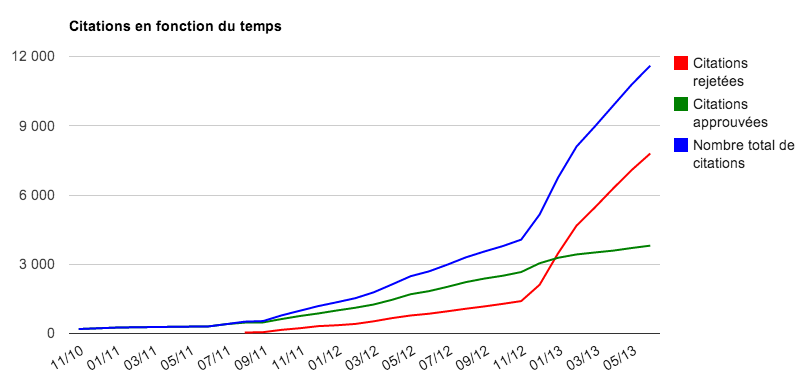
\includegraphics[width=450px]{images/statutsQuotesTemps.png}
		\caption{Nombre de citations acceptées et refusées en fonction du temps.}
	\end{figure}

	\begin{figure}[H]
		\center
		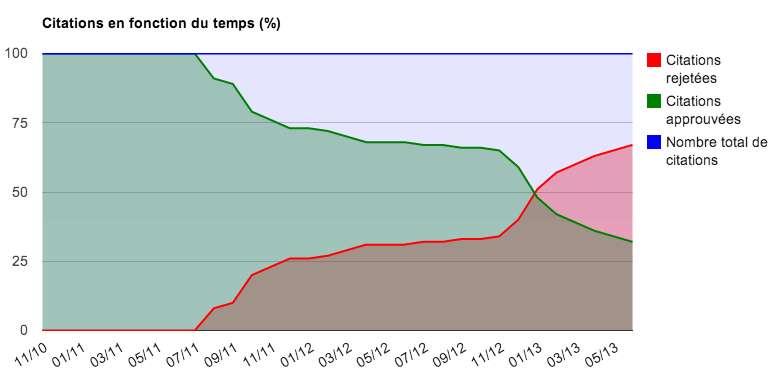
\includegraphics[width=450px]{images/statutsQuotesTempsPourcentage.png}
		\caption{Pourcentage de citations acceptées et refusées en fonction du temps.}
	\end{figure}
	
	La courbe (ou l'aire) bleue est la somme des courbes (ou des aires) bleues. 

	On remarque que la courbe verte est quasiment confondue avec la courbe bleue au lancement de Teen Quotes. Ceci s'explique par le fait qu'il était difficile de lancer Teen Quotes sans un contenu initial et une base d'utilisateurs quasi vide. Ainsi, il était habituel que je soumette et « m'auto-approuve » des quotes afin de proposer du contenu aux premiers visiteurs.\\

	Le nombre de quotes approuvées suit une croissance quasi linéaire depuis la création du site. En effet, le nombre de quotes postées par jour est quasiment constant à 5.\\

	En revanche, on remarque qu'à partir du mois de novembre 2012, le nombre de quotes refusées augmente énormément. Ceci s'explique par une hausse du nombre de soumissions de quotes (engendrée par une hausse du nombre de créations de comptes, mais nous le verrons plus loin !). Ce fort afflux de quotes a engendré beaucoup de refus car il n'était pas possible de publier toutes les quotes soumises. En conséquence, la modération des quotes soumises est très stricte depuis cette période car le nombre de quotes proposées est beaucoup plus important qu'auparavant.

	% ----------------------------------- %
	% -- Vous allez vite en besogne --- %
	\section{Vous allez vite en besogne}
	Un jour, j'ai eu une super idée : j'ai voulu savoir combien de temps après leur inscription les utilisateurs qui ont soumis des quotes ont soumis leur première quote. Il faut savoir que 40 \% des utilisateurs possédant un compte sur Teen Quotes ont déjà soumis au moins une quote. Il semblerait donc qu'une motivation importante pour créer un compte soit celle de pouvoir soumettre une quote. Vérifions ceci !

	\begin{figure}[H]
		\center
		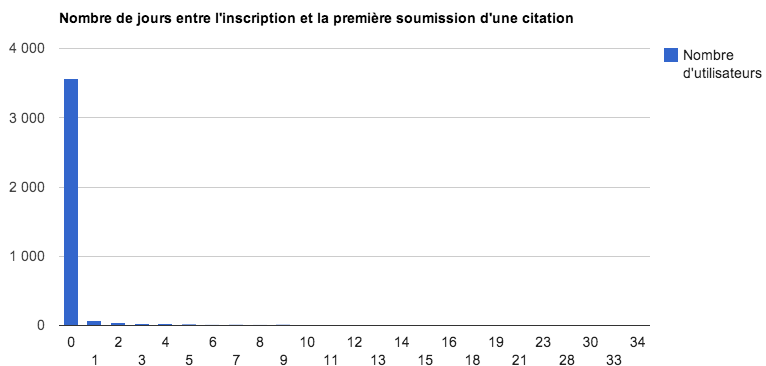
\includegraphics[width=450px]{images/inscriptionSoumissionQuote.png}
		\caption{Nombre de jours entre l'inscription et la première soumission d'une citation.}
	\end{figure}
	Pour obtenir les données nécessaires à la construction de ce graphique, voici l'idée suivie par l'algorithme :
	\vspace{10px}
	\begin{enumerate}
		\item On détermine tous les comptes ayant soumis au moins une quote. Pour chaque compte trouvé, on enregistre sa date d'inscription à Teen Quotes.
		\item Pour chaque compte trouvé précédemment, on détermine la première citation soumise.
		\item On calcule le nombre de jours entre la soumission de la première quote et la date de création du compte.
		\item On enregistre dans une grande matrice le nombre de jours entre l'inscription et la première soumission de quote et le nombre de comptes ayant ce nombre de jours.
		\item On élimine les lignes où il y a moins de 5 comptes qui ont soumis des citations au bout d'un nombre X de jours (que l'on note comme points aberrants).
	\end{enumerate}
	\vspace{10px}
	Interprétons ceci maintenant :
	\vspace{10px}
	\begin{itemize}
		\item Constat sans appel : une écrasante majorité des utilisateurs ayant soumis des citations le font pour la première fois moins de 24 heures après avoir créé leur compte sur Teen Quotes. Notre hypothèse se confirme : la création du compte est bien souvent motivée par l'envie de soumettre une citation.
		\item Au delà de 5 jours d'écarts entre l'inscription et la soumission de la première quote, on retrouve très peu de comptes : à chaque fois moins de 20 comptes sont concernés.  
	\end{itemize}
	\vspace{10px}
	Le détail des données est disponible sur \url{http://statistics.teen-quotes.com}. Il est intéressant de regarder les valeurs précises car il est difficile de se rendre compte de l'importance des cas hors épure sur le graphique présenté ci-dessus.

	% ------------------------------------------- %
	% -- Petits floodeurs ou gros floodeurs ? --- %
	\section{Petits floodeurs ou gros floodeurs ?}
	On rappelle la définition d'un \textit{floodeur} d'après Wikipédia.
	\begin{quote}
		\textit{Flood} est un anglicisme désignant une inondation, illustrant ainsi le flux de données ininterrompu et excessif transitant sur le réseau, provoquant alors des dégâts. Il a donné un verbe, \textit{flooder}, et la personne qui \textit{floode} est un \textit{floodeur}.
	\end{quote}

	\begin{figure}[H]
		\center
		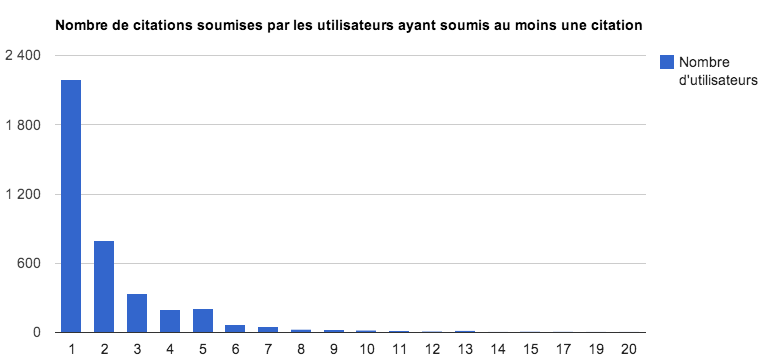
\includegraphics[width=450px]{images/citationsSoumisesParUtilisateur.png}
		\caption{Nombre de citations soumises par les utilisateurs ayant soumis au moins une citation.}
	\end{figure}
	Le processus pour obtenir les données nécessaires à l'obtention de ce graphique est très similaire au processus précédent.
	\vspace{10px}
	\begin{enumerate}
		\item On détermine tous les comptes ayant soumis au moins une quote. Pour chaque compte trouvé, on enregistre sa date d'inscription à Teen Quotes.
		\item Pour chaque compte trouvé précédemment, on compte le nombre de citations soumises.
		\item On enregistre dans une grande matrice le nombre de citations soumises et le nombre de comptes ayant ce nombre de citations.
	\end{enumerate}
	\vspace{10px}
	J'ai choisi de ne pas éliminer les points aberrants ici pour se rendre compte de la différence énorme entre l'épure des données et les points limites. Une fois de plus, le détail des données est disponible sur \mbox{\url{http://statistics.teen-quotes.com}}. Il est intéressant de regarder les valeurs précises car il est difficile de se rendre compte de l'importance des cas hors épure sur le graphique présenté ci-dessus.
	Interprétons ceci maintenant :
	\vspace{10px}
	\begin{itemize}
		\item Une écrasante majorité des gens ayant soumis des citations en soumettent moins de 5.
		\item Au delà de 10 citations soumises, on retrouve très peu de comptes : à chaque fois moins de 20 comptes sont concernés. La valeur maximale (493 citations soumises !) est attribuée à mon compte. Ceci s'explique par le fait que j'ai beaucoup contribué à remplir la base de données au lancement du site pour avoir un premier contenu sur Teen Quotes. 
	\end{itemize}
	\vspace{10px}

	% /////////////////////////////////////////// %
	% /// Les utilisateurs sont nos amis //////// %
	\chapter{Les utilisateurs sont nos amis}
	Intéressons-nous maintenant au coeur de ce qui compose Teen Quotes : \barre{du code !} les comptes \mbox{d'utilisateurs}. 

	% --------------------------------------- %
	% -- Plus on est de fous, plus on rit --- %
	\section{Plus on est de fous, plus on rit}
	Dans un premier temps observons l'évolution du nombre de comptes créés sur Teen Quotes au cours du temps. Pour faire ceci, l'algorithme suivi est le suivant :
	\vspace{10px}
	\begin{enumerate}
		\item On définit une variable correspond au 1er jour du mois de la création de Teen Quotes.
		\item On incrémente cette variable symbolisant le temps d'un mois, et on compte dans la table des comptes de Teen Quotes combien de comptes ont été créés avec une date d'inscription inférieure à celle-ci.
		\item On répète le processus jusqu'au premier du mois courant en enregistrant dans une matrice à chaque étape la date à laquelle on s'intéresse et le nombre de comptes s'étant inscrits avant cette date. 
	\end{enumerate}
	\vspace{10px}
	La requête SQL\footnote{SQL (sigle de \textit{Structured Query Language}, en français langage de requête structurée) est un langage informatique normalisé servant à effectuer des opérations sur des bases de données relationnelles. La partie langage de manipulation de données de SQL permet de rechercher, d'ajouter, de modifier ou de supprimer des données dans les bases de données relationnelles.} qu'il faut exécuter à chaque tour de boucle est la suivante :
	\begin{lstlisting}
		SELECT COUNT(id) AS nb_members 
		FROM teen_quotes_account 
		WHERE UNIX_TIMESTAMP(joindate) <= '$timestamp_calcule'
	\end{lstlisting}
	où la variable \texttt{\$timestamp\_calcule} est la date calculée au format timestamp\footnote{La valeur représentant la date et l'heure est appelée timestamp (de l'anglais \textit{time}, « heure » et \textit{stamp}, marquage par un timbre ou un tampon) ou tout simplement « horodatage ». Il peut s'agir d'une séquence de caractères (groupe date-heure) représentant la date et l'heure sous une forme intelligible. En informatique, ce type de format est souvent utilisé dans les journaux d'événements. Un timestamp peut aussi désigner un compteur numérique représentant une quantité de temps écoulée depuis un instant de référence, comme dans le système de l'heure Unix. Le timestamp se distingue alors de la date et de l'heure entendues comme un ensemble de valeurs année/mois/jour et heure/minute/seconde, la conversion pouvant se faire de l'un à l'autre.} UNIX.
	\begin{figure}[H]
		\center
		\includegraphics[width=450px]{images/membresTemps.png}
		\caption{Création de comptes utilisateurs en fonction du temps.}
	\end{figure}
	Sur ce graphique on a représenté la période de développement entre novembre 2010 et mai 2011. Sans surprise le nombre d'inscriptions pour cette période est quasiment nul et correspond à quelques « privilégiés » qui ont eu accès à Teen Quotes avant le lancement en mai 2011.

	De mai 2011 à novembre 2012 on observe une croissance quasi linéaire pour la création de comptes.

	De novembre 2012 jusqu'à juin 2013 on observe une croissance se rapprochant d'une exponentielle, ralentie vers les derniers mois. Cette croissance fulgurante coïncide à la sortie de l'application iPhone / iTouch.\\

	Tentons d'appliquer une régression pour se rapprocher de cette courbe. De toute évidence, il est inutile de tenter de modéliser la totalité de la courbe par modèle linéaire. Tentons une régression exponentielle de la forme $e^{ax + b}$.
	\begin{figure}[H]
		\center
		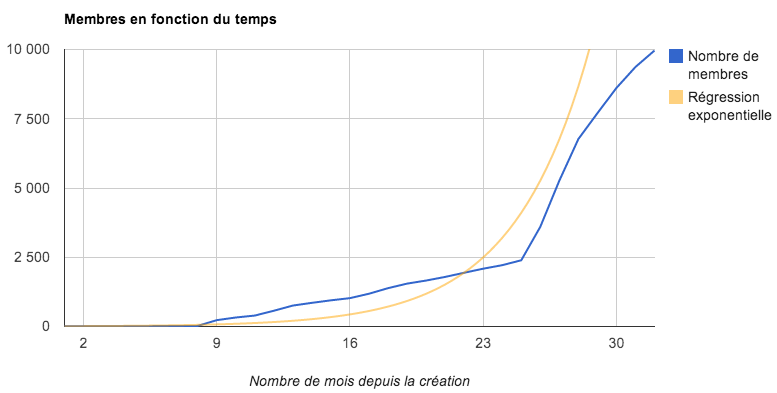
\includegraphics[width=450px]{images/membresRegression.png}
		\caption{Création de comptes utilisateurs en fonction du temps.}
	\end{figure}
	Comme on ne peut pas faire une régression avec comme abscisse des dates au format (MM/AA), on va transformer l'abscisse en indiquant le nombre de mois depuis la création de Teen Quotes.\\
	La meilleure régression exponentielle est donnée par :
	\[y = e^{0,249x + 2,093}\]
	Soit les coefficients suivants :
	\[\widehat{a} = 0,249\]
	\[\widehat{b} = 2,093\]

	% --------------------------------------- %
	% -- Déclinez votre âge je vous prie ---- %
	\section{Déclinez votre âge je vous prie}
	Intéressons-nous maintenant à l'âge des utilisateurs. Notre audience cible est les adolescents (c'est pour ça que l'on s'appelle \textbf{Teen} Quotes). Vérifions immédiatement si c'est bien le public visé qui visite Teen Quotes.\\

	Pour obtenir les données, l'algorithme suivi est le suivant :
	\vspace{10px}
	\begin{enumerate}
		\item On détermine tous les utilisateurs ayant renseigné leur date de naissance
		\item Pour chaque utilisateur on calcule son âge à la date actuelle.
		\item On enregistre dans une matrice l'âge et le nombre de comptes qui ont cet âge à la date actuelle.
	\end{enumerate}
	\vspace{10px}
	\begin{figure}[H]
		\center
		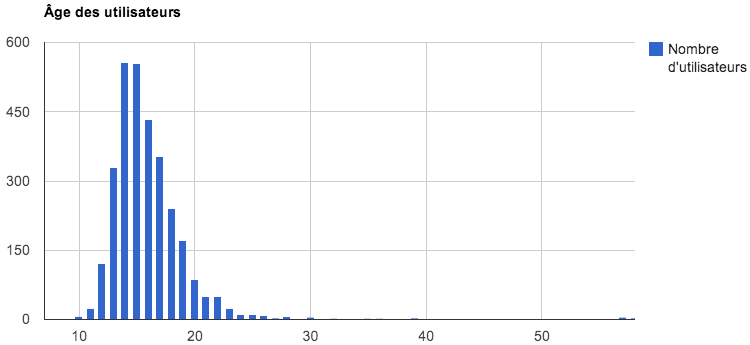
\includegraphics[width=450px]{images/ageUtilisateurs.png}
		\caption{Âge des utilisateurs de Teen Quotes.}
	\end{figure}
	On remarque immédiatement que l'âge des utilisateurs de Teen Quotes suit une loi normale, centrée entre 14 et 15 ans. 84 \% des utilisateurs de Teen Quotes ont entre 12 et 18 ans. Bonne nouvelle, l'audience visée est bien celle qui visite Teen Quotes !\\

	Comme d'habitude, le détail des données est disponible sur \url{http://statistics.teen-quotes.com}. Il est intéressant de regarder les valeurs précises car il est difficile de se rendre compte de l'importance des cas hors épure sur le graphique présenté ci-dessus.

	On peut tenter d'expliquer les cas lointains (plus de 50 ans) par des personnes d'un âge plus avancé qui s'identifient également aux citations publiées ou par des saisies incorrectes d'utilisateurs qui souhaitent modifier leur âge (ou qui se sont trompés).

	% --------------------------------------- %
	% -- Je veux voir ta bouille ------------ %
	\section{Je veux voir ta bouille}
	Sur Teen Quotes, il est bien évidemment possible de changer son avatar dès que l'on a un compte. Par défaut, un avatar est attribué à tous les utilisateurs ayant créé un compte. Intéressons-nous à la proportion d'utilisateurs ayant changé l'avatar proposé par défaut.
	\begin{figure}[H]
		\center
		
\includegraphics{images/avatarDefaut.png}
		\caption{L'avatar proposé par défaut aux utilisateurs de Teen Quotes.}
	\end{figure}

	\begin{figure}[H]
		\center
		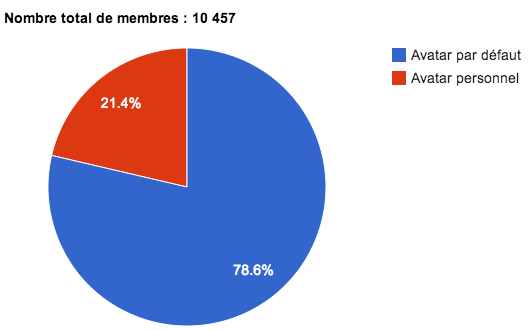
\includegraphics[width=300px]{images/partAvatar.png}
		\caption{Proportion des utilisateurs ayant modifié l'avatar attribué par défaut.}
	\end{figure}
	Environ $\frac{1}{5}$ des utilisateurs de Teen Quotes ont souhaité modifier leur avatar.

	% --------------------------------------- %
	% -- Pour vivre heureux, vivons cachés -- %
	\section{Pour vivre heureux, vivons cachés}
	Par défaut, lorsque quelqu'un crée un compte sur Teen Quotes, son profil est public. Tout visiteur peut alors consulter son profil, les citations dont il est auteur qui ont été approuvées, les citations que cet utilisateur a ajouté à ses favoris et les informations personelles que l'utilisateur a renseigné (pays, ville, date de naissance, biographie).\\

	Sur Teen Quotes, il est possible de cacher son profil. Intéressons-nous à la part d'utilisateurs qui ont souhaité rendre leur profil privé.

	\begin{figure}[H]
		\center
		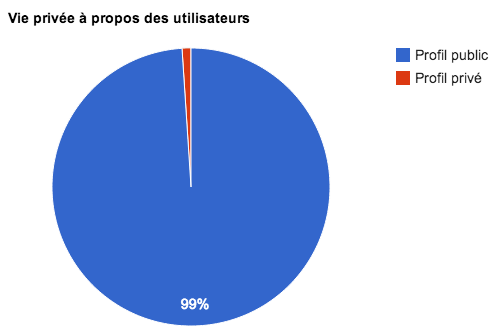
\includegraphics[width=280px]{images/viePriveeUtilisateurs.png}
		\caption{Proportions d'utilisateurs ayant un profil public et un profil privé.}
	\end{figure}

	Seulement 1 \% des utilisateurs ont choisi de rester dans l'anonymat.

	% /////////////////////////////////////////// %
	% /// Juste un petit commentaire //////////// %
	\chapter{Juste un petit commentaire}
	Il est temps d'en venir à un autre sujet important de Teen Quotes : les commentaires. Les commentaires sont stratégiques car ils représentent une partie du degré d'interaction des utilisateurs.

	Des utilisateurs qui commentent beaucoup sont des utilisateurs qui intéragissent avec Teen Quotes. L'objectif avec les commentaires est de pousser les utilisateurs à naviguer entre les quotes pour suivre les discussions, voire à revenir dans quelques heures ou quelques jours pour voir si la discussion a avancé.

	% ------------------------------------------------------------ %
	% -- Les mots s'envolent, mais les écrits restent ------------ %
	\section{Les mots s'envolent, mais les écrits restent}
	À la même manière que pour les comptes, intéressons-nous au nombre de commentaires qui ont été postés au cours du temps. L'algorithme suivi pour récupérer les données est le même que précédemment, sauf qu'on s'intéresse cette fois-ci aux commentaires et non aux comptes.\\

	Comme précédemment, on représente les quelques mois de développement qui ont précédé le lancement de Teen Quotes.
	\begin{figure}[H]
		\center
		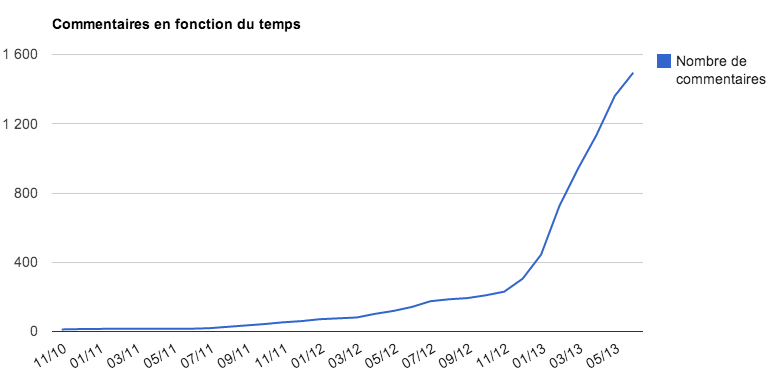
\includegraphics[width=450px]{images/commentairesTemps.png}
		\caption{Commentaires postés en fonction du temps sur Teen Quotes.}
	\end{figure}
	Ho ! Je connais cette courbe, elle ressemble étrangement à celle que l'on a obtenu précédemment quand on représentait le nombre de comptes au cours du temps. On retrouve les mêmes tendances pour les mêmes périodes :
	\vspace{10px}
	\begin{itemize}
		\item Une stagnation du nombre de commentaires durant la période de développement (novembre 2010 - mai 2011)
		\item Une augmentation quasi linéaire du nombre de commentaires entre mai 2011 et novembre 2012.
		\item Une croissance exponentielle du nombre de commentaires, qui semble moins ralentie que la croissance du nombre de comptes à partir de novembre 2012, lors de la sortie de l'application iPhone / iTouch.
	\end{itemize}
	\vspace{10px}
	Par ailleurs, cette croissance du nombre de commentaires à partir du mois novembre 2012 coïncide avec un changement d'interface qui a été bénéfique au nombre de commentaires postés. Précédemment, lorsqu'il y avait des commentaires sur une citation, il était indiqué le nombre de commentaire avec un petite texte.\\

	Nous avons choisi maintenant d'indiquer le nombre de commentaires dans une bulle bleue qui se remarque dès qu'il y avait au moins un commentaire et de garder l'affichage discret quand il n'y a pas de commentaires sur une citation. Nous avons attendu la sortie de l'application iPhone / iTouch pour mettre en production ce changement pour garder une interface unie sur la version classique, la version optimisée pour les mobiles et l'application iOS (les mises à jour d'une application étant beaucoup moins faciles à réaliser que sur les autres plateformes).
	\begin{figure}[H]
		\center
		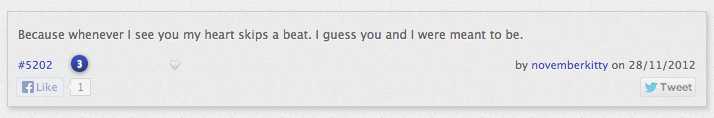
\includegraphics[width=470px]{images/quoteCommentaires.png}
		\caption{Une quote avec 3 commentaires sur la version classique.}
	\end{figure}
	\begin{figure}[H]
		\center
		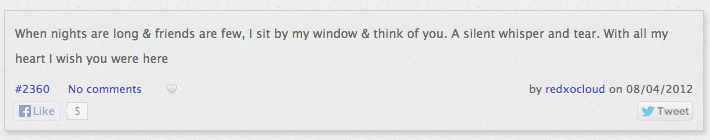
\includegraphics[width=470px]{images/quoteSansCommentaires.png}
		\caption{Une quote sans commentaires sur la version classique.}
	\end{figure}
	Tentons de réaliser une régression exponentielle sur la courbe obtenue.
	\begin{figure}[H]
		\center
		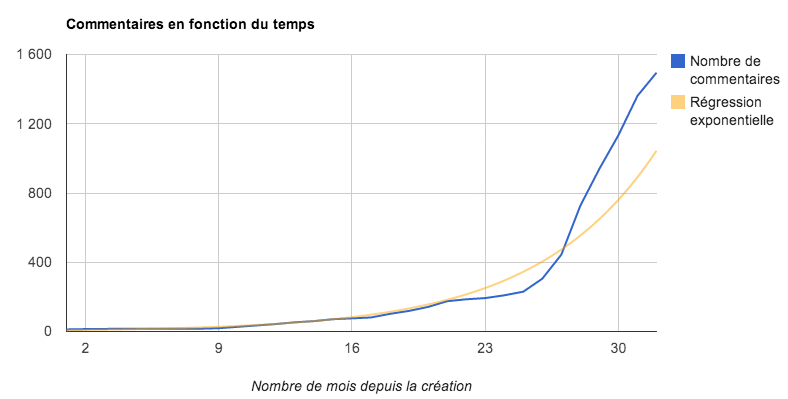
\includegraphics[width=450px]{images/commentairesRegression.png}
		\caption{Commentaires postés en fonction du temps sur Teen Quotes.}
	\end{figure}
	La meilleure régression exponentielle ($e^{ax + b}$) est donnée par :
	\[y = e^{0,158x + 1,885}\]
	Soit les coefficients suivants :
	\[\widehat{a} = 0,158\]
	\[\widehat{b} = 1,885\]

	% ----------------------------------------------------------- %
	% -- Un petit mot vaut mieux qu'un long discours ------------ %
	\section{Un petit mot vaut mieux qu'un long discours}
	Qu'est-ce qui est mieux : la briéveté d'un commentaire court ou le développement d'une idée contenue dans un commentaire plus long ? Il n'y a pas de bonne ou de mauvaise réponse, chacun se fera son propre avis. Observons comment se comportent les visiteurs de Teen Quotes dès qu'ils prennent \barre{leur plume} leur clavier pour écrire des mots.\\

	Voici la requête SQL qui nous permet de récupérer une matrice contenant les différentes longueurs des commentaires et le nombre de commentaires qui font chaque longueur trouvée.

	\begin{lstlisting}
		SELECT COUNT(*) AS nb, LENGTH(texte) AS length
		FROM teen_quotes_comments 
		GROUP BY LENGTH(texte)
		ORDER BY `nb` DESC
	\end{lstlisting}

	\begin{figure}[H]
		\center
		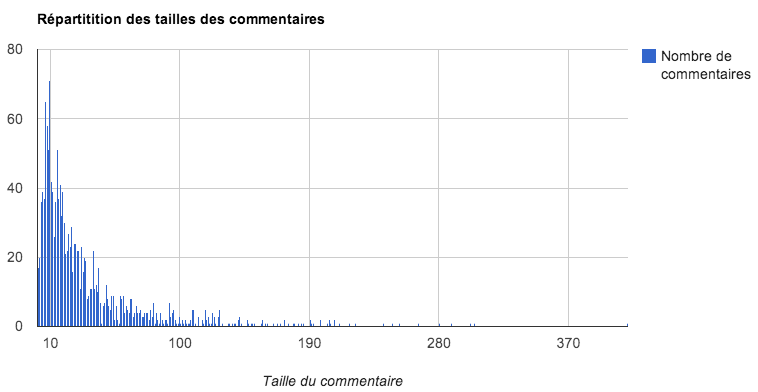
\includegraphics[width=470px]{images/tailleCommentaires.png}
		\caption{Taille des commentaires en nombre de caractères sur Teen Quotes.}
	\end{figure}

	On remarque immédiatement que les utilisateurs se sont entendus pour écrire des commentaires courts, voire très courts. Difficile d'exprimer une idée forte en moins de 20 caractères ! Notons que la taille du commentaire le plus long sur Teen Quotes est de 411 caractères, ce qui n'est pas un commentaire si long en soi.\\

	Allons plus loin et tentons de savoir combien de commentaires utilisent au moins le mot \textit{true}, en reprenant le slogan de Teen Quotes : \textit{Because some quotes are simply true}. La requête SQL est la suivante :
	\begin{lstlisting}
		SELECT COUNT(id) 
		FROM teen_quotes_comments
		WHERE text LIKE '%true%'
	\end{lstlisting}
	On obtient 327 commentaires, soit 20 \% des commentaires à l'heure où j'écris ce rapport ! On ne peut pas dire que le niveau de langue soit très développé dans les commentaires sur Teen Quotes.\\
		
	Encore une fois, le détail des données est disponible sur \url{http://statistics.teen-quotes.com}. Il est intéressant de regarder le tableau des différentes valeurs obtenues, tant l'ensemble des valeurs est grand.

	% /////////////////////////////////////////// %
	% /// Créer un compte : mode d'emploi /////// %
	\chapter{Créer un compte : mode d'emploi}
	Nous avons vu précédemment que, de temps en temps, des visiteurs créaient des comptes sur Teen Quotes. Mais comment en sont-ils arrivés jusqu'à là ? OK, nous n'allons pas nous plaindre, mais il serait bien d'en savoir un petit peu plus sur le processus qui a amené un visiteur à franchir le pas de la création d'un compte.

	% ----------------------------------------------------- %
	% -- Encore une histoire de lieu d'inscription -------- %
	\section{Encore une histoire de lieu d'inscription}
	La première question que l'on se pose naturellement est le lieu d'inscription de l'utilisateur. Combien de visiteurs créent un compte depuis l'application iOS ? Depuis le site classique ? Depuis le site web mobile ?\\

	Il est facile de connaître la réponse à cette question : il suffit d'enregistrer dans une colonne d'où a été effectuée la requête quand on insère une nouvelle ligne dans la table des comptes lors d'une inscription. La requête SQL pour récupérer les données est la suivante :
	\begin{lstlisting}
		SELECT COUNT(*) AS tot, location_signup
		FROM teen_quotes_account 
		GROUP BY location_signup 
		ORDER BY tot DESC
	\end{lstlisting}
	Représentons ceci sur un diagramme circulaire :
	\begin{figure}[H]
		\center
		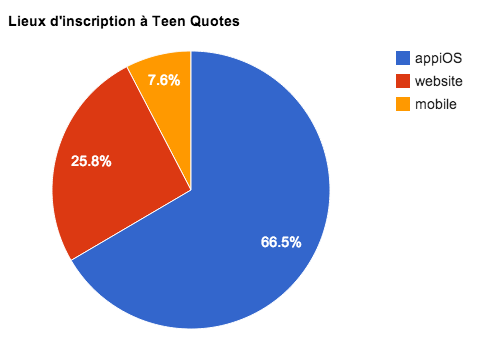
\includegraphics[width=300px]{images/lieuInscription.png}
		\caption{Lieux d'inscription des utilisateurs à Teen Quotes.}
	\end{figure}
	Les résultats sont étonnants : alors que l'application iOS est sortie en novembre 2012, \textbf{plus de 66 \% du total des comptes ont été créés depuis celle-ci}.\\

	L'application, développée initialement pour répondre aux usages des visiteurs de Teen Quotes (une grande partie d'entre eux utilisant un mobile sous iOS) a eu un autre effet : nous avons réussi à capter d'autres visiteurs, qui n'étaient pas réceptifs aux médias où nous étions disponibles auparavant (web et web mobile). Ce public, utilisateur d'applications, est plus intéressé par une application native sous iOS que par un accès à une version mobile ou depuis un ordinateur.\\

	Ceci confirme bien que notre objectif est important : nous n'arriverons pas à faire converger toutes les personnes intéressées par le concept de Teen Quotes vers un seul média. Il est donc nécessaire de proposer plusieurs moyens de suivre et de participer à Teen Quotes (réseaux sociaux, site web, web mobile, applications) pour pouvoir agrandir notre base d'utilisateurs.

	% ------------------------------------------- %
	% -- Comment êtes-vous arrivés ici ? -------- %
	\section{Comment êtes-vous arrivés ici ?}
	Concentrons-nous maintenant au site web et au site mobile. Pourquoi sur ceux-ci ? Car il est beaucoup plus facile techniquement de mettre en place des outils d'analyse personnalisés. Nous allons chercher à savoir comment les utilisateurs peuvent arriver sur la page d'inscription.\\

	Plusieurs chemins menant vers la page d'inscription sont possibles :
	\vspace{10px}
	\begin{itemize}
		\item L'utilisateur a cliqué sur le lien menant vers l'inscription dans le menu placé en haut.
		\item L'utilisateur a cliqué sur le lien menant vers l'inscription placé en bas du formulaire de connexion, placé sur la droite du site.
		\item L'utilisateur voulait ajouter une citation et a été redirigé vers la page d'inscription.
		\item L'utilisateur voulait ajouter un commentaire et a été redirigé vers la page d'inscription.
		\item L'utilisateur a accédé directement à la page d'inscription ou il ne rentre dans aucun des cas précédents.
	\end{itemize}
	\vspace{10px}
	\paragraph{Explication supplémentaire :}nous avons choisi de mettre le lien d'ajout d'une citation, même si le visiteur n'était pas connecté car nous avons vu précédemment que la motivation première pour créer un compte était l'envie d'ajouter une citation. En conséquence, on place un lien qui semble méner à l'ajout d'une citation, qui redirige en réalité vers l'inscription, pour essayer de créer l'envie de s'inscrire de l'utilisateur.\\

	Les détails techniques pour détecter les différents chemins d'inscription ne seront pas détaillés ici\footnote{Voir le chapitre \ref{chap:ressources} « Ressources » page \pageref{chap:ressources} pour plus d'informations.}.\\

	Sans plus attendre, présentons les résultats :
	\begin{figure}[H]
		\center
		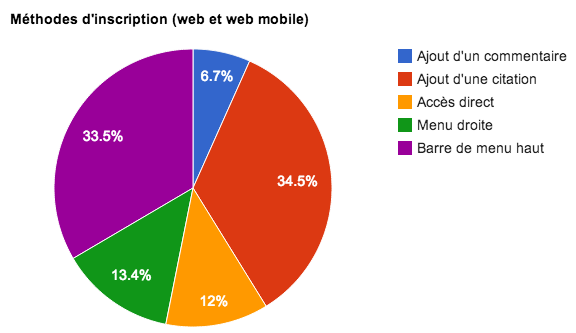
\includegraphics[width=300px]{images/methodesDInscription.png}
		\caption{Méthodes d'inscription des utilisateurs à Teen Quotes (web et web mobile).}
	\end{figure}
	Interprétons immédiatement les résultats obtenus :
	\vspace{10px}
	\begin{itemize}
		\item Les résultats confirment notre impression : autant d'utilisateurs sont arrivés sur la page d'inscription en souhaitant ajouter une citation qu'en souhaitant s'inscrire de leur plein gré (en cliquant sur le lien dans la barre de menu placée en haut).
		\item On remarque également qu'aucune méthode n'est manifestement minoritaire : il était donc important de proposer plusieurs possibilités pour arriver finalement à la page d'inscription.
	\end{itemize}
	\vspace{10px}
	 
	% /////////////////////////////////////////// %
	% /// Technologies utilisées //////////////// %
	\chapter{Technologies utilisées}
	Un bon projet ne se fait pas sans bonne technologie, avec des langages de programmation puissants et des outils performants.\\

	Voici la liste des langages de programmation utilisés :
	\vspace{10px}
	\begin{itemize}
		\item \texttt{PHP} : logique métier.
		\item \texttt{SQL} : accès aux données dans les bases de données.
		\item \texttt{HTML} : interface homme-machine, structure hiérarchique du contenu.
		\item \texttt{CSS} : mise en forme / design des contenus web.
		\item \texttt{JavaScript} : amélioration de l'expérience utilisateur.
		\item \LaTeX\ : rédaction du présent rapport.
	\end{itemize}
	\vspace{10px}

	Logiciels, bibliothèques et API\footnote{En informatique une interface de programmation (API pour \textit{Application Programming Interface}) est un ensemble normalisé de classes, des méthodes ou des fonctions qui sert de façade par laquelle un logiciel offre des services à d'autres logiciels. Elle est offerte par une bibliothèque logicielle ou un service web, le plus souvent accompagnée d'une description qui spécifie comment des programmes consommateurs peuvent se servir des fonctionnalités du programme fournisseur.}s utilisés :
	\vspace{10px}
	\begin{itemize}
		\item \texttt{Facebook API} : intégration d'outils de partage pour le réseau social.
		\item \texttt{Twitter API} : intégration d'outils de partage pour le réseau social.
		\item \texttt{CloudFlare} : CDN\footnote{Un \textit{Content Delivery Network} (CDN) est constitué d’ordinateurs reliés en réseau à travers Internet et qui coopèrent afin de mettre à disposition du contenu ou des données (généralement du contenu multimédia volumineux) à des utilisateurs.}, mise en cache des contenus, serveurs DNS.
		\item \texttt{MySQL} : système de gestion de bases de données.
		\item \texttt{Apache} : serveur HTTP utilisé pour le contenu non statique.
		\item \texttt{Nginx} : serveur web et proxy inverse utilisé sur le CDN.
		\item \texttt{Git} : gestionnaire de versions.
		\item \texttt{jQuery} :  bibliothèque JavaScript libre qui porte sur l'interaction entre JavaScript (comprenant Ajax) et HTML, et a pour but de simplifier des commandes communes de JavaScript.
		\item \texttt{Google Analytics} : outil d'analyse d'audience pour contenus web.
		\item \texttt{Flurry} : outil d'analyse d'audience pour applications iOS.
		\item \texttt{Google Chart API} : création de graphiques à partir de données calculées. Les graphiques sont calculées dans le navigateur de l'utilisateur final.
		\item \texttt{animate.css} : bibliothèque CSS pour les animations proposées sur Teen Quotes.
		\item \texttt{uniform.css} : bibliothèque CSS / JavaScript pour avoir des formulaires uniformisés sur Teen Quotes.
		\item \texttt{timeago.js} : plugin jQuery pour la gestion des dates relatives.
	\end{itemize}
	
	% /////////////////////////////// %
	% /// Ressources //////////////// %
	\chapter{Ressources}
	\label{chap:ressources}
	Teen Quotes est un projet open-source, c'est-à-dire que le code source de Teen Quotes est consultable et redistribuable sous les mêmes conditions de cette licence. Le code source de l'application iOS n'est pas placé sous cette licence et n'est pas consultable.\\

	\begin{itemize}
		\item Répertoire GitHub de Teen Quotes : \url{https://github.com/AntoineAug/Teen-Quotes/}
		\item Liste des changements effectués sur Teen Quotes : \url{https://github.com/AntoineAug/Teen-Quotes/commits/master}
		\item Fichiers spécifiques à la réalisation de ce rapport : \url{https://github.com/AntoineAug/Teen-Quotes/tree/master/statistics}
		\item Disponibilité de Teen Quotes : \url{http://uptime.teen-quotes.com/}
		\item Calcul des statistiques à intervalle de temps régulier : voir les fichiers \texttt{kernel/fonctions.php} entre les lignes 184 et 968 (fonction \texttt{update\_stats}) et \texttt{cron.php}.
	\end{itemize}

	\paragraph{Remarque :} plus de 4 000 lignes de code ont été nécessaires pour réaliser les graphiques présentés dans ce rapport et le partie web dédiée à l'affichage des statistiques. Tous les algorithmes utilisés pour calculer les données présentées ici sont consultables en suivant les liens ci-dessus.

	\begin{figure}[H]
		\center
		
\includegraphics[width=250px]{images/promoApp.png}
		\caption{Image de promotion utilisée lors de la sortie de l'application iOS de Teen Quotes.}
	\end{figure}

% Fin du document
\end{document}